\documentclass{article}
	\usepackage{graphicx}

	\begin{document}

	\title{HW/SW Entwurfssprachen am Beispiel System-C}
	\author{Florian Zaruba, Thomas Weber}

	\maketitle

	%\begin{abstract}
	%The abstract text goes here.
	%\end{abstract}

	\section{HW/SW Design Languages}
	tba
	\section{What is SystemC}
	tba
	  \subsection{History}
	  tba
	  \subsection{Benefits}
	  tba
	  \subsection{Drawbacks}
	  tba
	  \subsection{SysC vs. C}
	  tba
	  \subsection{SysC vs. VHDL}

	\section{Automatic Partitioning}
	  \subsection{What is Partitioning?}
	  Partitioning means the separation of hardware and software parts with focus on hardware/software co-design.
	  Traditionally the hardware part of an embedded system is written in VHDL \textit{(more present in Europe)} or Verilog \textit{(more present in the USA)} while the software part is written in \textit{assembly}, \textit{C} or \textit{C++}.
	  The common design-flow (depicted in Figure~\ref{fig:flow}) shows that partitioning splits the design in hardware and software.
	  The software part is the shorter one of this two paths because it needs only an compiler to translate it to machine-code. Therefore, the hardware part is the much longer way because of the hardware design-flow which is necessary for every chip-design.
	    \begin{figure}[hp]
	      \centering
	      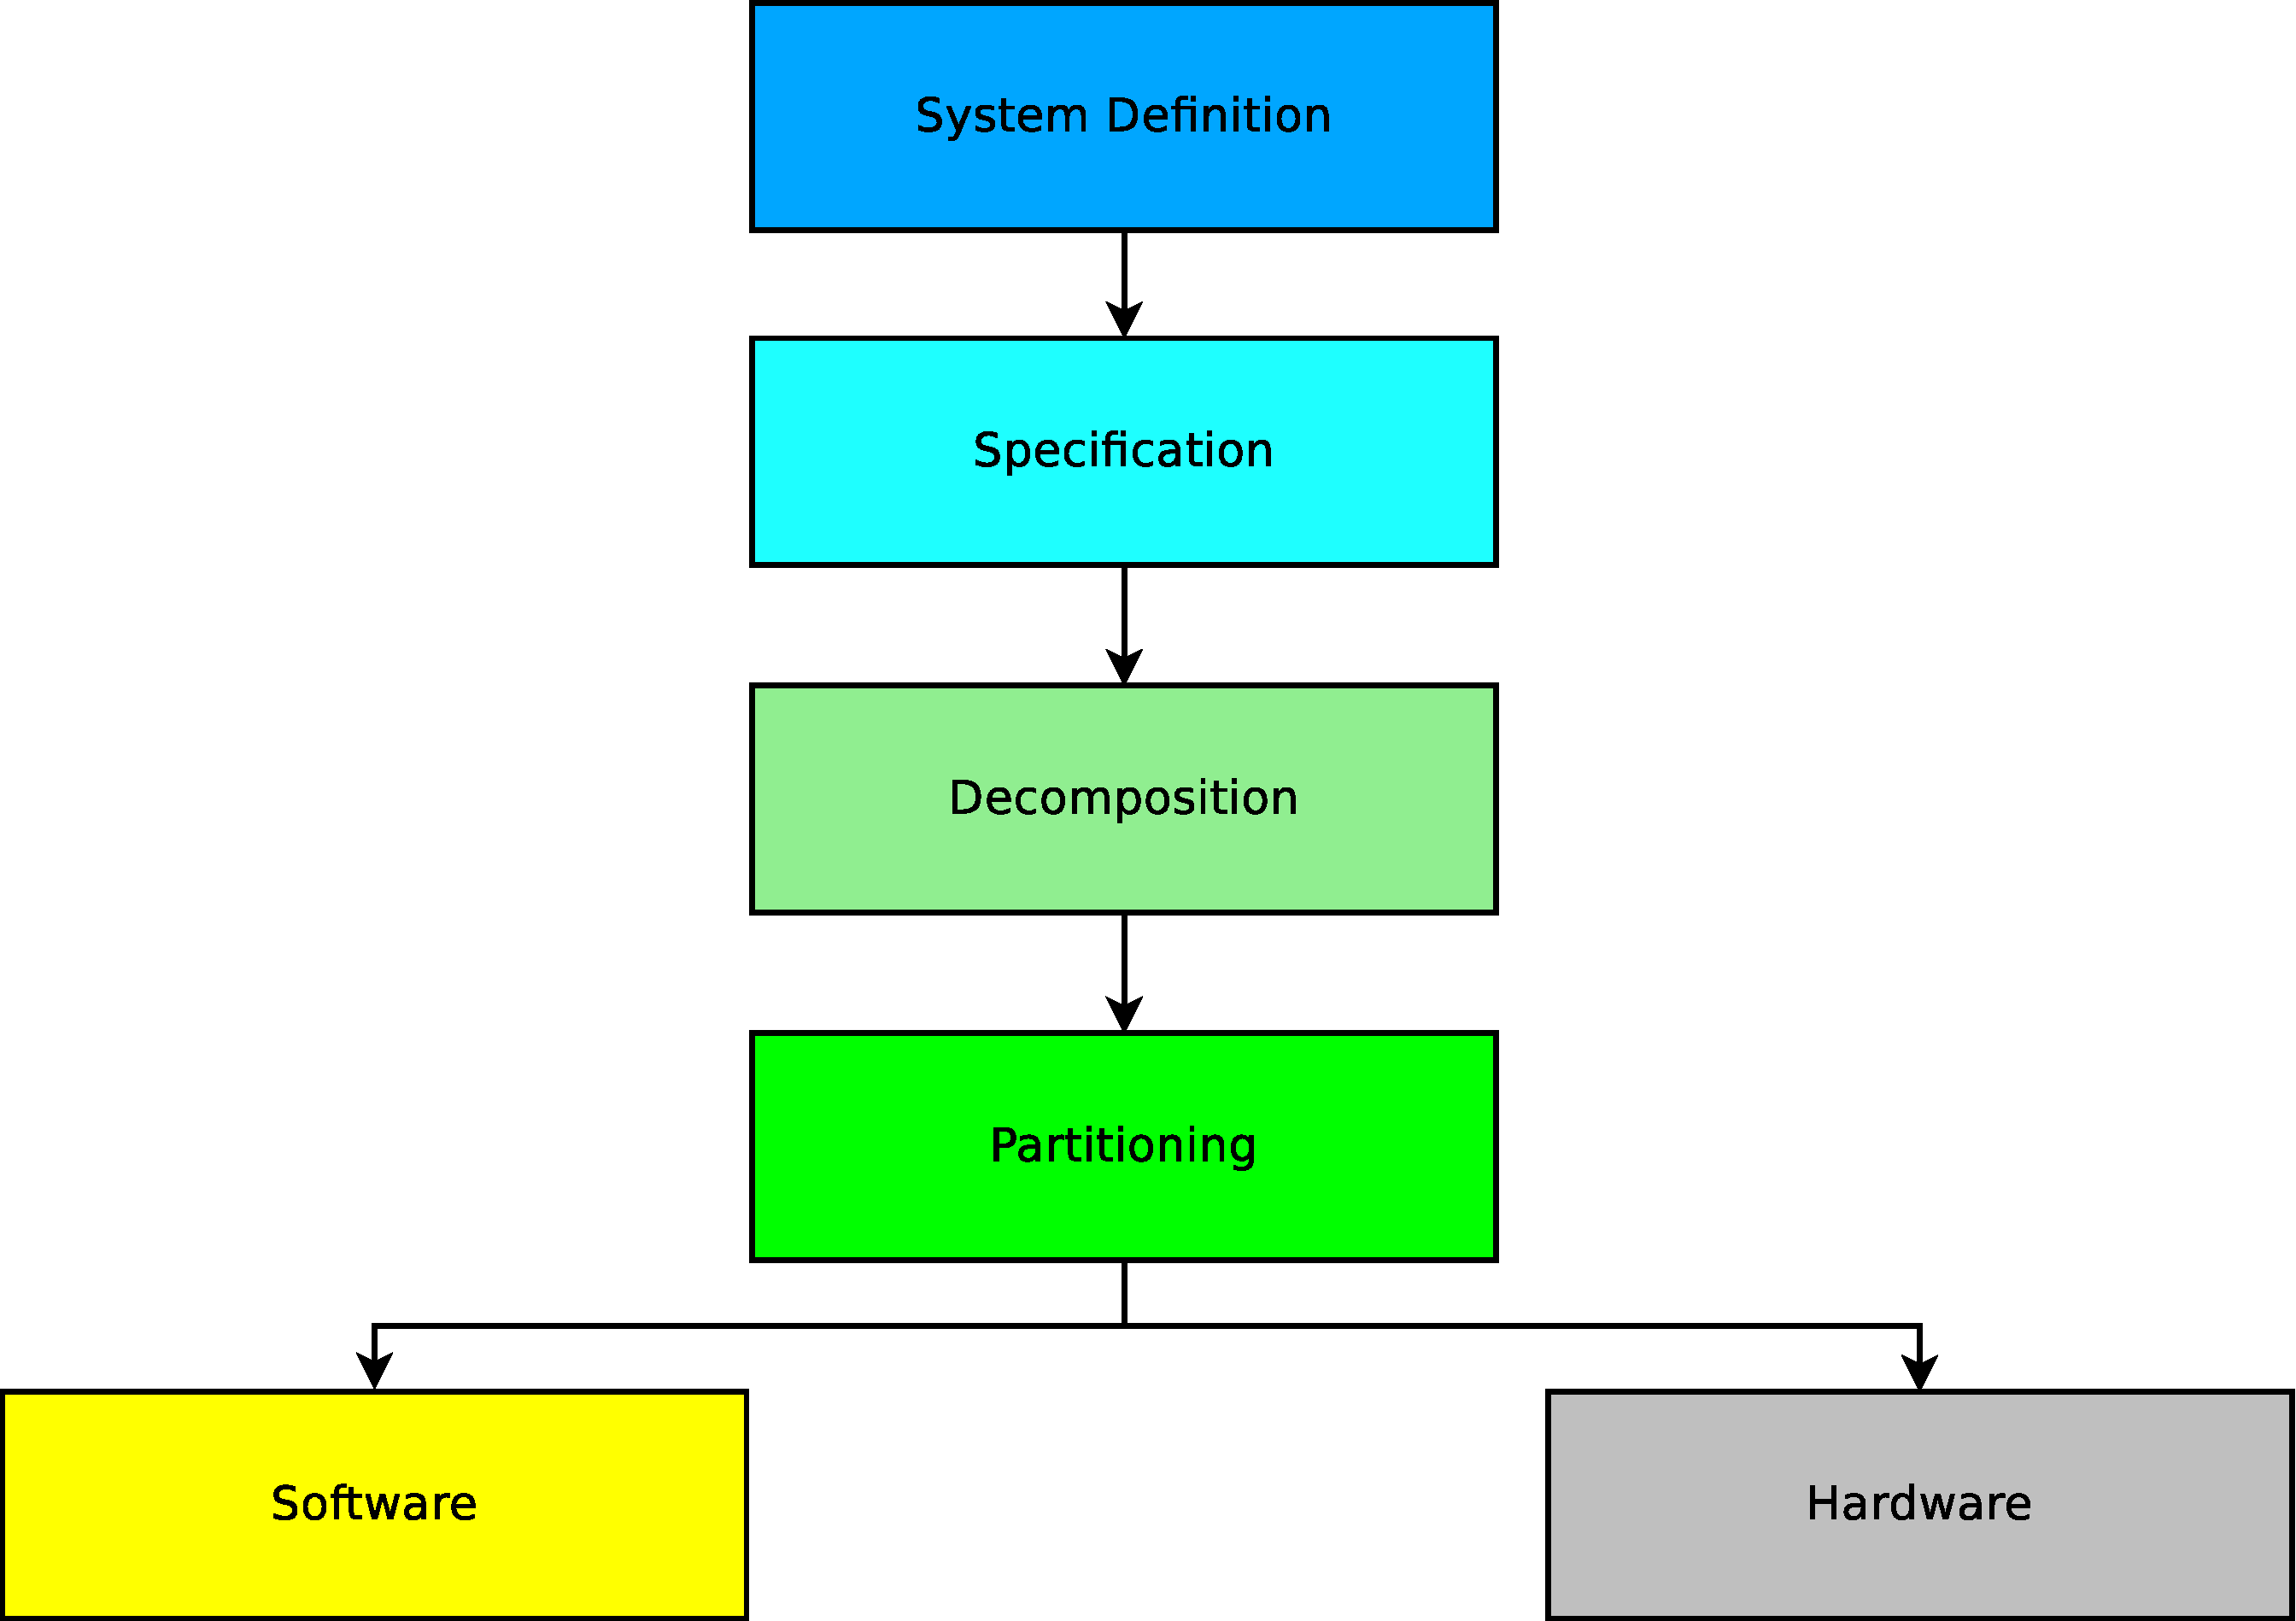
\includegraphics[scale=0.18]{../pictures/flow.pdf}
	      \caption{Design flow \textit{(c.f. Hardware Modelling VO)}.}
	      \label{fig:flow}
	    \end{figure}  
	  If the hardware and software parts should be modified because of, e.g., performance reasons, these two parts must be modified or completely redesigned in order to fit the specifications.
	  This leads to an much higher and probably expensive procedure for the hardware part, thus its design-flow is much longer and every change in the \textit{VHDL/Verilog} code leads to a new compilation, technology-mapping and place and route.
%	  Unless there are other circumstances, the \textit{system definition} and the \textit{specification} steps are part of the project management which have to be done only once.
	  \subsection{Tools for Automatic Partitioning}
	  
	\section{Tools}

	\section{Users}
	  \subsection{Accellera}
	  \subsection{ARM}
	    \begin{figure}[hp]
	      \centering
	      
\includegraphics[scale=0.18]{../pictures/armlogo.jpg}
	      \caption{ARM Ltd.}
	      \label{fig:arm}
	    \end{figure}  
	    ARM (Advanced RISC Machines) Ltd. has an active community\footnote{http://community.arm.com} and there are many informations about tools and IP cores available.
	    SystemC is used by many chip designers and they use the systemC-IP-cores from ARM Ltd. to simulate their designs.
	  \subsection{AMD}
	  
	  \subsection{Intel}
	  
\end{document}
